\documentclass[11pt,a4paper]{article}

% ============================================================================
% Language & Character Encoding
% ============================================================================
\usepackage[utf8]{inputenc}
\usepackage[T1]{fontenc}
\usepackage[english]{babel}

% ============================================================================
% Page Geometry & Spacing
% ============================================================================
\usepackage[a4paper,margin=2cm,top=2.8cm,bottom=2.5cm]{geometry}
\usepackage{amsmath,amssymb}
\usepackage{graphicx}
\usepackage{booktabs}
\usepackage{array}
\usepackage{tabularx}
\usepackage{fancyhdr}
\usepackage{lastpage}
\usepackage{xcolor}
\usepackage{hyperref}
\usepackage{float}
\usepackage{caption}

\hypersetup{
    colorlinks=true,
    linkcolor=blue!70!black,
    urlcolor=blue!70!black,
    pdftitle={EdgeSlice - Manual Calculation (Audited & Revised)}
}

% Color definitions for highlights
\definecolor{highlightred}{RGB}{180, 20, 20}
\definecolor{highlightgreen}{RGB}{20, 120, 40}
\definecolor{highlightblue}{RGB}{0, 70, 160}

% Header & Footer configuration
\pagestyle{fancy}
\fancyhf{}
\lhead{%
  \begin{tabular}{@{}l@{}}
    \textbf{Ho Chi Minh City University of Technology (HCMUT)} \\
    \textbf{Faculty of Computer Science and Engineering}
  \end{tabular}%
}
\rhead{}
\rfoot{\small Page \thepage/\pageref{LastPage}}
\renewcommand{\headrulewidth}{0.5pt}
\setlength{\headheight}{32pt}

\setlength{\parindent}{0pt}
\setlength{\parskip}{5pt}
\renewcommand{\arraystretch}{1.2}

\begin{document}

% ============================================================================
% SECTION 1: DAG STRUCTURE
% ============================================================================
\section{DAG Structure}

\begin{center}
\IfFileExists{DAG.jpg}{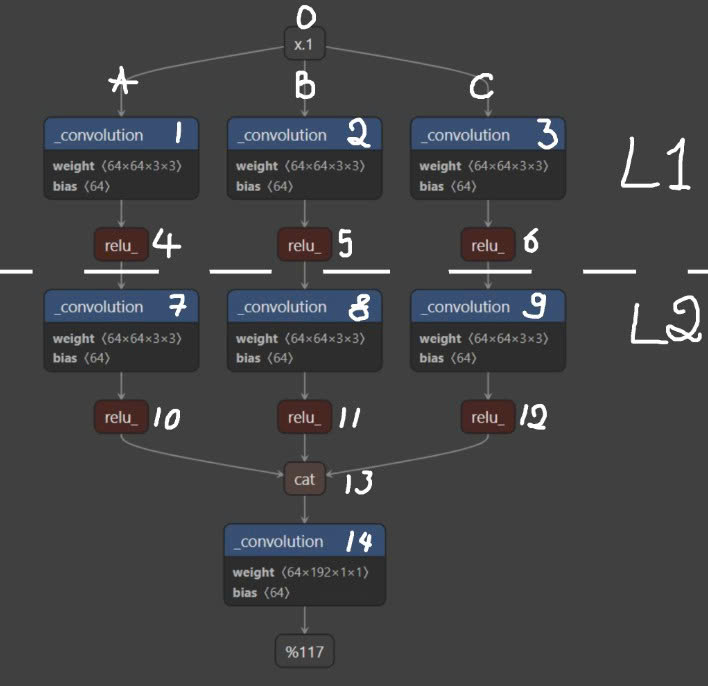
\includegraphics[width=0.7\textwidth]{DAG.jpg}}{%
\IfFileExists{graph.png}{\includegraphics[width=0.7\textwidth]{graph.png}}{%
  \fbox{\parbox{0.7\textwidth}{\centering\vspace{1.2cm}\textbf{[Figure 1: DAG]}\\\small(Please place \texttt{DAG.jpg} or \texttt{graph.png} in the document directory)\vspace{1.2cm}}}}}
\end{center}

\textbf{Input:} \texttt{x.1} --- shape $(1, 64, 56, 56)$

All Convolutions are configured with $\text{stride}=1$, $\text{dilation}=1$, $\text{kernel}=3$ (except the final Conv which is $1\times 1$).

\newpage

% ============================================================================
% SECTION 2: STAGE 1 - DAG CONSTRUCTION
% ============================================================================
\section{Stage 1: DAG Construction}

\subsection{Node Identification}

\begin{table}[H]
\centering
\small
\begin{tabular}{cllll}
\toprule
\textbf{Node ID} & \textbf{Op type} & \textbf{Input tensors} & \textbf{Output tensor} & \textbf{Params} \\
\midrule
0  & \texttt{x.1} (input placeholder)               & ---            & $(1, 64, 56, 56)$  & --- \\
1  & \texttt{linalg.conv\_2d\_nchw\_fchw} (Branch A, L1) & \texttt{x.1}, \texttt{W\_A1} & $(1, 64, 56, 56)$  & $\text{stride}=1, \text{dil}=1$ \\
2  & \texttt{linalg.conv\_2d\_nchw\_fchw} (Branch B, L1) & \texttt{x.1}, \texttt{W\_B1} & $(1, 64, 56, 56)$  & $\text{stride}=1, \text{dil}=1$ \\
3  & \texttt{linalg.conv\_2d\_nchw\_fchw} (Branch C, L1) & \texttt{x.1}, \texttt{W\_C1} & $(1, 64, 56, 56)$  & $\text{stride}=1, \text{dil}=1$ \\
4  & \texttt{linalg.elemwise\_unary} / ReLU (Branch A)   & \texttt{T1}          & $(1, 64, 56, 56)$  & $\text{op}=\text{relu}$ \\
5  & \texttt{linalg.elemwise\_unary} / ReLU (Branch B)   & \texttt{T2}          & $(1, 64, 56, 56)$  & $\text{op}=\text{relu}$ \\
6  & \texttt{linalg.elemwise\_unary} / ReLU (Branch C)   & \texttt{T3}          & $(1, 64, 56, 56)$  & $\text{op}=\text{relu}$ \\
7  & \texttt{linalg.conv\_2d\_nchw\_fchw} (Branch A, L2) & \texttt{T4}, \texttt{W\_A2}  & $(1, 64, 56, 56)$  & $\text{stride}=1, \text{dil}=1$ \\
8  & \texttt{linalg.conv\_2d\_nchw\_fchw} (Branch B, L2) & \texttt{T5}, \texttt{W\_B2}  & $(1, 64, 56, 56)$  & $\text{stride}=1, \text{dil}=1$ \\
9  & \texttt{linalg.conv\_2d\_nchw\_fchw} (Branch C, L2) & \texttt{T6}, \texttt{W\_C2}  & $(1, 64, 56, 56)$  & $\text{stride}=1, \text{dil}=1$ \\
10 & \texttt{linalg.elemwise\_unary} / ReLU (Branch A)   & \texttt{T7}          & $(1, 64, 56, 56)$  & $\text{op}=\text{relu}$ \\
11 & \texttt{linalg.elemwise\_unary} / ReLU (Branch B)   & \texttt{T8}          & $(1, 64, 56, 56)$  & $\text{op}=\text{relu}$ \\
12 & \texttt{linalg.elemwise\_unary} / ReLU (Branch C)   & \texttt{T9}          & $(1, 64, 56, 56)$  & $\text{op}=\text{relu}$ \\
13 & \texttt{tensor.concat} / cat                        & \texttt{T10, T11, T12} & $(1, 192, 56, 56)$ & $\text{dim}=1$ \\
14 & \texttt{linalg.conv\_2d\_nchw\_fchw} ($1\times 1$ conv) & \texttt{T13}, \texttt{W\_fin} & $(1, 64, 56, 56)$  & $\text{stride}=1, \text{dil}=1$ \\
\bottomrule
\end{tabular}
\end{table}

\subsection{Topological Order (Kahn's Algorithm + Min-Heap)}

Topological order: $[0, 1, 2, 3, 4, 5, 6, 7, 8, 9, 10, 11, 12, 13, 14]$

% ============================================================================
% SECTION 3: STAGE 2 - LIVENESS ANALYSIS
% ============================================================================
\section{Stage 2: Liveness Analysis}

\subsection{Tensor Size Calculation}

We have $\text{Float32} = 4\text{ bytes/element}$ ($1\text{ word} = 4\text{ bytes}$).

\textbf{Tensor Sizes:}
\begin{itemize}
    \item $T_{\text{input}}$ (\texttt{x.1}): $1 \times 64 \times 56 \times 56 \times 4 = 802,816\text{ bytes} \sim 784\text{ KB}$
    \item $T_1 = T_2 = T_3$: $1 \times 64 \times 56 \times 56 \times 4 = 802,816\text{ bytes} \sim 784\text{ KB}$
    \item $T_4 = T_5 = T_6$: $1 \times 64 \times 56 \times 56 \times 4 = 802,816\text{ bytes}$
    \item $T_7 = T_8 = T_9$: $1 \times 64 \times 56 \times 56 \times 4 = 802,816\text{ bytes}$
    \item $T_{10} = T_{11} = T_{12}$: $1 \times 64 \times 56 \times 56 \times 4 = 802,816\text{ bytes}$
    \item $T_{13}$ (\texttt{cat} output): $1 \times 192 \times 56 \times 56 \times 4 = 2,408,448\text{ bytes} \sim 2.3\text{ MB}$
    \item $T_{14}$ (final output): $1 \times 64 \times 56 \times 56 \times 4 = 802,816\text{ bytes}$
\end{itemize}

\textbf{Weights:}
\begin{itemize}
    \item $W_{Ax} / W_{Bx} / W_{Cx}$ (L1, L2): $64 \times 64 \times 3 \times 3 \times 4 = 147,456\text{ bytes}$
    \item $W_{\text{fin}}$ ($1\times 1$ conv): $64 \times 192 \times 1 \times 1 \times 4 = 49,152\text{ bytes}$
\end{itemize}

\newpage

\subsection{Computation of $p(t)$ and $\ell(t)$ for Intermediate Tensors}

\begin{table}[H]
\centering
\begin{tabular}{llll}
\toprule
\textbf{Tensor} & \textbf{Producer ($p$)} & \textbf{Consumers} & $\boldsymbol{\ell(t) = \max(\text{consumers})}$ \\
\midrule
$T_{\text{input}}$ & 0  & $\{1, 2, 3\}$ & 3 \\
$T_1$              & 1  & $\{4\}$       & 4 \\
$T_2$              & 2  & $\{5\}$       & 5 \\
$T_3$              & 3  & $\{6\}$       & 6 \\
$T_4$              & 4  & $\{7\}$       & 7 \\
$T_5$              & 5  & $\{8\}$       & 8 \\
$T_6$              & 6  & $\{9\}$       & 9 \\
$T_7$              & 7  & $\{10\}$      & 10 \\
$T_8$              & 8  & $\{11\}$      & 11 \\
$T_9$              & 9  & $\{12\}$      & 12 \\
$T_{10}$             & 10 & $\{13\}$      & 13 \\
$T_{11}$             & 11 & $\{13\}$      & 13 \\
$T_{12}$             & 12 & $\{13\}$      & 13 \\
$T_{13}$             & 13 & $\{14\}$      & 14 \\
$T_{14}$             & 14 & $\{\}$ (sink) & 14 \\
\bottomrule
\end{tabular}
\end{table}

\subsection{Live Tensors at Each Program Point (Audited against EdgeSlice Code)}

Tensor $t$ is alive at program point $i$ if and only if: $p(t) \le i \le \ell(t)$

\begin{table}[H]
\centering
\small
\begin{tabular}{clc}
\toprule
\textbf{Point $\boldsymbol{i}$} & \textbf{Live Tensors (Active in Memory)} & \textbf{Total Bytes} \\
\midrule
0  & $T_{\text{input}}$                                                                 & 802,816 \\
1  & $T_{\text{input}}, T_1$                                                             & 1,605,632 \\
2  & $T_{\text{input}}, T_1, T_2$                                                         & 2,408,448 \\
3  & $T_{\text{input}}, T_1, T_2, T_3$                                                     & 3,211,264 \\
4  & $T_1, T_2, T_3, T_4$ \quad \textcolor{gray}{\small($T_{\text{input}}\to\text{dead}$)} & 3,211,264 \\
5  & $T_2, T_3, T_4, T_5$ \quad \textcolor{gray}{\small($T_1\to\text{dead}$)}             & 3,211,264 \\
6  & $T_3, T_4, T_5, T_6$ \quad \textcolor{gray}{\small($T_2\to\text{dead}$)}             & 3,211,264 \\
7  & $T_4, T_5, T_6, T_7$ \quad \textcolor{gray}{\small($T_3\to\text{dead}$)}             & \textbf{3,211,264} \\
8  & $T_5, T_6, T_7, T_8$ \quad \textcolor{gray}{\small($T_4\to\text{dead}$)}             & \textbf{3,211,264} \\
9  & $T_6, T_7, T_8, T_9$ \quad \textcolor{gray}{\small($T_5\to\text{dead}$)}             & \textbf{3,211,264} \\
10 & $T_7, T_8, T_9, T_{10}$ \quad \textcolor{gray}{\small($T_6\to\text{dead}$)}            & \textbf{3,211,264} \\
11 & $T_8, T_9, T_{10}, T_{11}$ \quad \textcolor{gray}{\small($T_7\to\text{dead}$)}           & \textbf{3,211,264} \\
12 & $T_9, T_{10}, T_{11}, T_{12}$ \quad \textcolor{gray}{\small($T_8\to\text{dead}$)}          & \textbf{3,211,264} \\
13 & $T_{10}, T_{11}, T_{12}, T_{13}$ \quad \textcolor{gray}{\small($T_9\to\text{dead}$)}     & \textbf{4,816,896} \textbf{\textcolor{highlightred}{(Global Peak)}} \\
14 & $T_{13}, T_{14}$ \quad \textcolor{gray}{\small($T_{10}, T_{11}, T_{12}\to\text{dead}$)}    & \textbf{3,211,264} \\
\bottomrule
\end{tabular}
\end{table}

\textbf{\textcolor{highlightblue}{* Audit Notes and Revisions vs. Initial Draft:}}
\begin{enumerate}
    \item \textbf{Points 4, 5, 6:} $T_{\text{input}}$ has no consumers after Node 3 ($\ell(T_{\text{input}}) = 3$); hence at $i=4$, $T_{\text{input}}$ is already deallocated. Conversely, $T_1$ is currently read by Node 4, meaning $T_1$ remains alive at $i=4$. The exact live set at Point 4 is $\{T_1, T_2, T_3, T_4\}$.
    \item \textbf{Points 7 to 12:} Node 7 reads $T_4$ to produce $T_7$; thus at $i=7$, $T_4$ is still alive ($p(T_4)\le 7 \le \ell(T_4)=7$). The true live set consists of 4 tensors ($3,211,264\text{ B}$), rather than 3 tensors ($2,408,448\text{ B}$).
    \item \textbf{Point 13 (\texttt{cat} operator):} Throughout the execution of Op 13, all 3 input tensors ($T_{10}, T_{11}, T_{12}$) and the output tensor $T_{13}$ must reside simultaneously in memory: $(3 \times 802,816) + 2,408,448 = \mathbf{4,816,896\text{ bytes}} \approx \mathbf{4.59\text{ MB}}$. This represents the true \textbf{Global Peak Memory} of the whole model graph.
    \item \textbf{Point 14 (Conv $1\times 1$):} Op 14 reads $T_{13}$ and generates $T_{14}$; therefore, memory occupancy is $2,408,448 + 802,816 = \mathbf{3,211,264\text{ bytes}}$ (not $802,816\text{ B}$).
\end{enumerate}

% ============================================================================
% SECTION 4: STAGE 3 - CANDIDATE SELECTION
% ============================================================================
\section{Stage 3: Candidate Selection}

$$\text{Budget} = 512\text{ KB} \times 80\% = 409,600\text{ bytes}$$

\paragraph{Conv L1 (nodes 1, 2, 3)}
\begin{align*}
\text{op\_type} &= \texttt{conv\_2d\_nchw\_fchw} \\
\text{output shape} &: (1, 64, 56, 56) \\
\text{input shape} &: (1, 64, 56, 56) \\
\text{weight shape} &: (64, 64, 3, 3)
\end{align*}
Full working set:
\begin{align*}
\text{output} &: 1 \times 64 \times 56 \times 56 \times 4 = 802,816\text{ bytes} \\
\text{input} &: 1 \times 64 \times 56 \times 56 \times 4 = 802,816\text{ bytes} \\
\text{weight} &: 64 \times 64 \times 3 \times 3 \times 4 = 147,456\text{ bytes} \\
\midrule
\text{Total} &: 1,753,088\text{ bytes} \sim 1.67\text{ MB}
\end{align*}
$1,753,088 > \text{Budget} \implies$ \textbf{Tile (Candidate)}

\paragraph{ReLU (nodes 4--6, 10--12)}
$$\text{Full working set} = \text{output} + \text{input} = 2 \times 802,816 = 1,605,632\text{ bytes}$$
$1,605,632 > \text{Budget} \implies$ \textbf{Tile (Candidate)}

\paragraph{Conv L2 (nodes 7--9)}
$$\text{Total} = 1,753,088\text{ bytes} > \text{Budget} \implies \textbf{Tile (Candidate)}$$

\paragraph{Cat (node 13)}
\texttt{tensor.concat} is a data movement operation, not a compute \texttt{linalg} operator (\texttt{is\_tileable} exclusion).
$\implies$ \textbf{Do Not Tile}

\paragraph{Final Conv (node 14)}
\begin{align*}
\text{output} &: 1 \times 64 \times 56 \times 56 \times 4 = 802,816\text{ bytes} \\
\text{input} &: 1 \times 192 \times 56 \times 56 \times 4 = 2,408,448\text{ bytes} \\
\text{weight} &: 64 \times 192 \times 1 \times 1 \times 4 = 49,152\text{ bytes} \\
\midrule
\text{Total} &: 3,260,416\text{ bytes} \sim 3.11\text{ MB}
\end{align*}
$3,260,416 > \text{Budget} \implies$ \textbf{Tile (Candidate)}

\paragraph{Final Candidate List}

\begin{table}[H]
\centering
\begin{tabular}{clcc}
\toprule
\textbf{Node} & \textbf{Op} & \textbf{Full WS (bytes)} & \textbf{Tile?} \\
\midrule
$1, 2, 3$   & Conv $3\times 3$ L1 & $1,753,088$ & \checkmark \\
$4, 5, 6$   & ReLU L1             & $1,605,632$ & \checkmark \\
$7, 8, 9$   & Conv $3\times 3$ L2 & $1,753,088$ & \checkmark \\
$10, 11, 12$ & ReLU L2             & $1,605,632$ & \checkmark \\
$13$         & cat                 & N/A         & $\times$ \\
$14$         & Conv $1\times 1$    & $3,260,416$ & \checkmark \\
\bottomrule
\end{tabular}
\end{table}

\newpage

% ============================================================================
% SECTION 5: STAGE 4 - DIMENSION SELECTION
% ============================================================================
\section{Stage 4: Dimension Selection}

Under EdgeSlice priority order for NCHW layout (dense convolution, batch=1):
$$\text{Spatial H} \succ \text{Spatial W} \succ \text{Channel}$$
$\implies$ \textbf{Prioritize slicing along the H dimension (\texttt{spatial\_h}) for both Conv and ReLU.}

% ============================================================================
% SECTION 6: STAGE 5 - TILE SIZE CALCULATION
% ============================================================================
\section{Stage 5: Tile Size Calculation}

$$\text{Budget} = 409,600\text{ bytes}$$

\subsection{Conv L1, L2}
$\text{shape} = (1, 64, 56, 56), \text{dim} = \texttt{spatial\_h}, \text{stride}=1, \text{dilation}=1, \text{kernel}=3$

\textbf{Output tile:}
$$(1, 64, T_h, 56) = 64 \times T_h \times 56 \times 4 = 14,336 \times T_h\text{ bytes}$$

Calculating required input height with spatial halo padding:
\begin{align*}
h_{\text{in}} &= (T_h - 1) \times \text{stride} + \text{dilation} \times (\text{kernel}_h - 1) + 1 \\
&= (T_h - 1) \times 1 + 1 \times 2 + 1 \\
&= T_h + 2 \quad (\text{Add 2 halo rows})
\end{align*}

\textbf{Input tile:}
$$(1, 64, T_h + 2, 56) = 64 \times (T_h + 2) \times 56 \times 4 = 14,336 \times (T_h + 2)\text{ bytes}$$

\textbf{Weight tile:}
$$(64, 64, 3, 3) \times 4 = 147,456\text{ bytes}$$

\textbf{Total footprint:}
\begin{align*}
F(T_h) &= 14,336 \times T_h + 14,336 \times (T_h + 2) + 147,456 \\
&= 28,672 \times T_h + 28,672 + 147,456 \\
&= 28,672 \times T_h + 176,128\text{ bytes}
\end{align*}

Enforcing capacity constraint $F(T_h) \le 409,600$:
$$28,672 \times T_h \le 233,472 \implies T_h \le 8.143$$
$\implies$ Optimal integer tile size is $T_h = 8$:
$$F(8) = 28,672 \times 8 + 176,128 = 229,376 + 176,128 = 405,504\text{ bytes} \le \text{Budget}$$

\textbf{With $T_h = 8$:}
\begin{itemize}
    \item Each tile produces $8\text{ output rows}$ and requires $10\text{ input rows}$ ($8 + 2\text{ halo}$).
    \item Number of tiles $= \lceil 56/8 \rceil = \mathbf{7\text{ tiles}}$.
\end{itemize}

\subsection{All ReLU Layers}
Analogously (no halo expansion and no weight parameters):
$$F(T_h) = 28,672 \times T_h$$
Constraint: $F(T_h) \le 409,600 \implies T_h \le 14.28 \implies \text{best: } T_h = 14 \xrightarrow{\text{align to power-of-2}} \mathbf{T_h = 8}$
\begin{itemize}
    \item Number of tiles $= \lceil 56/8 \rceil = \mathbf{7\text{ tiles}}$.
\end{itemize}

\newpage

\subsection{Final Conv (Node 14, Conv $1\times 1$)}
Analogously ($1\times 1$ pointwise conv requires no spatial halo):
\begin{align*}
\text{Input tile} &: (1, 192, T_h, 56) = 192 \times T_h \times 56 \times 4 = 43,008 \times T_h\text{ bytes} \\
\text{Output tile} &: (1, 64, T_h, 56) = 64 \times T_h \times 56 \times 4 = 14,336 \times T_h\text{ bytes} \\
\text{Weight tile} &: (64, 192, 1, 1) \times 4 = 49,152\text{ bytes} \\
\midrule
F(T_h) &= (43,008 + 14,336) \times T_h + 49,152 = 57,344 \times T_h + 49,152\text{ bytes}
\end{align*}
Constraint: $57,344 \times T_h + 49,152 \le 409,600 \implies 57,344 \times T_h \le 360,448 \implies T_h \le 6.285$.
$$\text{best: } T_h = 6 \xrightarrow{\text{align to power-of-2}} \mathbf{T_h = 4}$$
Tile size for Final Conv: $\mathbf{T_h = 4}$ \\
Number of tiles $= \lceil 56/4 \rceil = \mathbf{14\text{ tiles}}$

% ============================================================================
% SECTION 7: STAGE 6 - SCHEDULE SEARCH
% ============================================================================
\section{Stage 6: Schedule Search}

Given 1D cascade search and 1 legal dimension per op:

\begin{table}[H]
\centering
\begin{tabular}{clccc}
\toprule
\textbf{Node} & \textbf{Op} & \textbf{Slice dim} & \textbf{Tile size} & \textbf{Tiles} \\
\midrule
$1, 2, 3$   & Conv $3\times 3$ L1 & H & 8 & 7 \\
$4, 5, 6$   & ReLU L1             & H & 8 & 7 \\
$7, 8, 9$   & Conv $3\times 3$ L2 & H & 8 & 7 \\
$10, 11, 12$ & ReLU L2             & H & 8 & 7 \\
$14$         & Conv $1\times 1$    & H & 4 & 14 \\
\bottomrule
\end{tabular}
\end{table}

% ============================================================================
% SECTION 8: STAGE 7 - FUSION PLANNING
% ============================================================================
\section{Stage 7: Fusion Planning}

\subsection{Fusion Chains}
Final anchors:
\begin{itemize}
    \item $\{1, 2, 3\}$ (Conv L1 per branch)
    \item $\{7, 8, 9\}$ (Conv L2 per branch; ReLU L1 is fused into here)
    \item $\{10, 11, 12\}$ (ReLU L2)
    \item $\{14\}$ (Conv $1\times 1$)
\end{itemize}

\subsection{Re-fit Tile Size after Fusion}
\textbf{Group members:}
Node 7 (Conv L2) + Node 4 (ReLU\_A1)

\textbf{Group total footprint:}
\begin{align*}
F_{\text{group}}(T_h) &= F_{\text{Conv L2}}(T_h) + F_{\text{ReLU}}(T_h) \\
&= (28,672 \times T_h + 176,128) + 28,672 \times T_h \\
&= 57,344 \times T_h + 176,128\text{ bytes}
\end{align*}
Constraint: $57,344 \times T_h + 176,128 \le 409,600 \implies 57,344 \times T_h \le 233,472 \implies T_h \le 4.071$.
$$\text{best: } T_h = 4 \xrightarrow{\text{align}} \mathbf{T_h = 4}$$

\textbf{Tile size after fusion:}
\begin{table}[H]
\centering
\begin{tabular}{clccc}
\toprule
\textbf{Node} & \textbf{Op} & \textbf{Slice dim} & \textbf{Tile size} & \textbf{Tiles} \\
\midrule
$1, 2, 3$   & Conv $3\times 3$ L1       & H & 8 & 7 \\
$7, 8, 9$   & Conv $3\times 3$ L2 fused & H & 4 & 14 \\
$10, 11, 12$ & ReLU L2                   & H & 8 & 7 \\
$14$         & Conv $1\times 1$          & H & 4 & 14 \\
\bottomrule
\end{tabular}
\end{table}

\newpage

% ============================================================================
% SECTION 9: STAGE 8 - MLIR TRANSFORM IR GENERATION
% ============================================================================
\section{Stage 8: MLIR Transform IR Generation}

\textit{This transformation script is automatically synthesized by the EdgeSlice compiler (\texttt{SlicedRewrite.generate\_transform\_ir()}). Manual calculation is impractical due to SSA handle chaining, \texttt{transform.structured.match}, \texttt{tile\_using\_forall}, and \texttt{fuse\_into\_containing\_op} transformations.}

% ============================================================================
% SECTION 10: MEMORY TIERS (AUDITED & REVISED)
% ============================================================================
\section{Memory Tiers}

\begin{table}[H]
\centering
\begin{tabular}{ll}
\toprule
\textbf{Op} & \textbf{Tile Working Set (Memory Tier)} \\
\midrule
Conv L1 (tile $H=8$)       & $405,504\text{ B} \approx 396\text{ KB}$ \\
Conv L2 fused (tile $H=4$) & $405,504\text{ B} \approx 396\text{ KB}$ \\
ReLU L2 (tile $H=8$)       & $14,336 \times 8 \times 2 = 229,376\text{ B} \approx 224\text{ KB}$ \\
Conv $1\times 1$ (tile $H=4$) & $\mathbf{278,528\text{ B} \approx 272\text{ KB}}$ \textsuperscript{(*)} \\
\bottomrule
\end{tabular}
\end{table}

\textsuperscript{(*)} \textbf{\textcolor{highlightblue}{Audit Note:}} \\
The initial draft recorded $393,216\text{ B} \approx 384\text{ KB}$, which was the pre-aligned footprint of $T_h = 6$ ($57,344 \times 6 + 49,152 = 393,216\text{ B}$). Once the tile size is rounded to $T_h = 4$, the true working set of Conv $1\times 1$ is:
$$F(4) = 57,344 \times 4 + 49,152 = \mathbf{278,528\text{ bytes}} \approx \mathbf{272\text{ KB}}$$

\end{document}
